\chapter{Background}

\todo{introductory text, easing into this chapter}



Computers need electricity to compute. 
This electricity is usually sourced from the public and local grid, which in turn is made up of many different energy producers. This energy mix is composed of different sources: low-carbon technologies like solar, wind, or hydroelectricity and carbon-intensive sources like coal, gas, or oil.

Over the day, the demand and supply for power changes. For example, during the midday, solar is produced as the sun shines. In the morning or evening hours however, as people may enjoy a cup of coffee or watch television, additional 

Thus, at each point in time the amount of CO2 per unit of electric power can be determined by averaging the amount of power each source supplies to the grid and how much carbon it emits.

\begin{itemize}
    \item power grid is made up of different sources
    \item these sources have a varying amount of carbon per unit of power (solar is efficient, while burning oil is not)
    \item this mix changes throughout the day, solar power can only be produced as the sun shines, burning fossile fuel can be done whenever and is needed to supply the base load.
    \item carbon-aware scheduling thus assumes that, if we schedule our jobs during low carbon periods, we emit less CO2 for the same amount of work
    \item this only works for deferrable or batch workloads \cite{tanenbaum_operating_2006}
    \item secondary benefits such as potentially a lower cost using dynamic energy prices
\end{itemize}


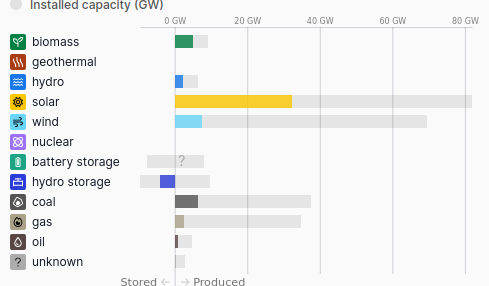
\includegraphics[width=\linewidth]{images/2_background2024-08-20-15-28-19.png}

\section*{Types of Carbon Aware Scheduling}
    - There are different ways to exploit the dynamic carbon emissions: temportal shifting, spatial, ressource scaling.
    - what do we focus on in this thesis and why?


\section*{Different Signals of the grid}

\begin{itemize}
    \item marginal and relative carbon
    \item what does each signal mean for making decisions? 
    \item why do we use the relative signal? \todo{there was some discussion about that in my bib; if we point to that it'll surely be fine}
\end{itemize}

hintergrund energie netz, stormproduktion
welche arten davon gibt es 
welche benefits hat das?
hintergrund signals nach denen entschieden wird (marinal / relative carbon)
welche metriken gibt es POI-A, etc etc.
\begin{itemize}
    \item energy is produced by different sources, leading to a different amount of carbon/unit of energy over time. 
    \item Welche Methoden gibt es carbon einzusparen (vllt. auch in der related work) (temporal, spatial, ressource scaling)
    \item Begründen warum sich das lohnen kann (marinal / relative carbon), kein wasting von erneuerbaren energien (losses among saving energy into batteries / "curtailment" !!)
    \item welche metriken gibt es POI-A, etc etc.
    \item Jobs <-> dynamic ernergie verbrauch, wie wird sowas gemessen?
\end{itemize}